\documentclass[a4paper,14pt]{extarticle}
\def\source{/home/osabio/tex/templates}
\input{\source/head.tex}
\yakovlev{159}{Электростатика}
\begin{document}

\begin{figure}[H]
    \centering
    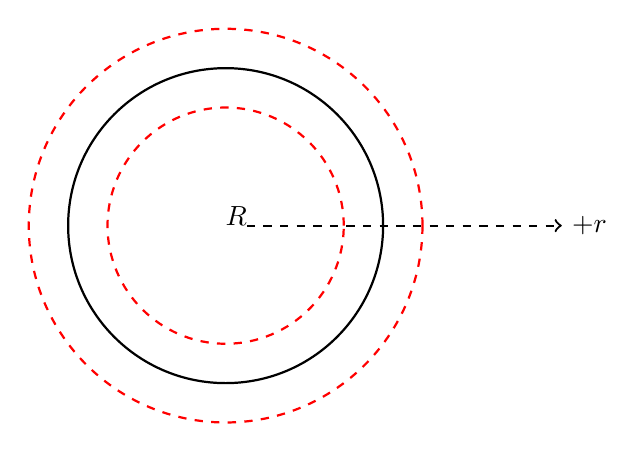
\begin{tikzpicture}
        \draw[thick] (0,0) circle (2cm); 
        \draw[thick, dashed, red] (0,0) circle (2.5cm); 
        \draw[thick, dashed, red] (0,0) circle (1.5cm); 
        \lineann[-4]{90}{2}{$R$};
        \draw[thick,->,dashed] (0,0) -- (4,0) node[right]{$+r$};
    \end{tikzpicture} 
\end{figure}
Найдем напряженность поля сферы по теореме Гаусса:
\begin{equation}
	\oiint\limits_{(S)}(\vec{E},d\vec{S})=k\cdot4\pi q_{in}
\end{equation}
\begin{equation}
	ES=E4\pi r^2=k\cdot4\pi\left\{
	\begin{aligned}
		&\frac43\pi R^3 \rho, & r<R\\
		&\frac43\pi r^3 \rho, & r\geq R
	\end{aligned}
	\right.
\end{equation}
Откуда
\begin{equation}
	E=\left\{
	\begin{aligned}
		&\frac43\pi \rho k r, & r<R\\
		&\frac43\pi \rho k \frac{R^3}{r^2}, & r\geq R
	\end{aligned}
	\right.
\end{equation}
Тогда плотность собственной энергии
\begin{equation}
	w=\frac{E^2}{8\pi k}=\left\{
	\begin{aligned}
		&\frac{kq^2r^2}{8\pi R^6}, & r<R\\
		&\frac{kq^2}{8\pi r^4}, & r\geq R
	\end{aligned}
	\right.
\end{equation}
Но тогда
\begin{gather}
	W=\iiint\limits_{(V)}w\,dV=
	\int\limits_0^R
	\frac{kq^2r^2}{8\pi R^6}
	4\pi r^2 dr
	+
	\int\limits_R^\infty
	\frac{kq^2}{8\pi r^4}
	4\pi r^2 dr=\\\nonumber=
	\frac{kq^2}{2 R^6}
\int\limits_0^R	
	 r^4 dr
	+
	\int\limits_R^\infty
	\frac{kq^2}{2r^2}
	dr=\frac{kq^2}{10R}+\frac{kq^2}{2R}=\frac{6kq^2}{10R}=\frac{3kq^2}{5R}
\end{gather}
% Пусть начальная емкость конденсатора $C_0$. Тогда
% \begin{equation}
% 	C_0=\frac{S}{k\cdot4\pi d}
% \end{equation}
% Расположим медную пластину на расстоянии $l$ внутри конденсатора. Тогда емкость между 1 и 2 будет
% \begin{equation}
% 	C_{12}=\frac{S}{k\cdot4\pi l}
% \end{equation}
% А между 2 и 3
% \begin{equation}
% 	C_{23}=\frac{S}{k\cdot4\pi (\frac34d-l)}
% \end{equation}

% Заменим систему эквивалентной, скомпонованной из конденсаторов:
% \begin{figure}[H]
%     \centering
% 	\begin{circuitikz}[scale=1.25, every node/.style={scale=1.25}]
% 		\draw (-2,0) node[anchor=east]{1}
%   		to[short, o-*] (0,0)
% 		% to[] ++(0,2) 
% 		to[C=$C_{12}$] ++(2,0)
% 		to ++(0,-2)
% 		to[C=$C_{23}$] ++(-2,0);
% 		\draw (-2,-2) node[anchor=east]{3}
%   		to[short, o-*] ++(2,0);
% 	\end{circuitikz}
% \end{figure}
% Общая емкость конденсаторов  $C_{12}$ и $C_{23}$
% \begin{equation}
% 	\frac{1}{C}=\frac{1}{C_{12}}+\frac{1}{C_{23}}=
% 	\frac{1}{S}\left[
% 		{k\cdot4\pi (\frac34d-l)}+
% 		{k\cdot4\pi l}
% 	\right]=\frac{k\cdot 3\pi d}{S}
% \end{equation}
% То есть
% \begin{equation}
% 	C=\frac{S}{k\cdot 3\pi d}=\frac43C_0
% \end{equation}
% \begin{equation}
% 	C-C_0=\frac13C_0=200 \text{ Пф}
% \end{equation}
% Как видно, положение листа $l$ не влияет на ответ (емкость увеличивается на треть). Важно, чтобы лист оставался параллелен обкладкам, тогда будут верны использованные при выводе формулы плоского конденсатора.

\end{document}